% --------------------------------------------------------------
% This is all preamble stuff that you don't have to worry about.
% Head down to where it says "Start here"
% --------------------------------------------------------------
 
\documentclass[english,12pt]{article}
%\usepackage[latin9]{inputenc}
\usepackage[T1]{fontenc}
\usepackage{amsmath, amsthm, amssymb}
\usepackage[ansinew]{inputenc}
\usepackage[margin=1in]{geometry}
\usepackage{float}
\usepackage{graphicx}
\usepackage{lmodern}
\usepackage{esint}
\usepackage{caption}
\usepackage{subcaption}
\usepackage[]{units}
\usepackage{listings}
\RequirePackage{hyperref} 
\usepackage{color} %red, green, blue, yellow, cyan, magenta, black, white
\definecolor{mygreen}{RGB}{28,172,0} % color values Red, Green, Blue
\definecolor{mylilas}{RGB}{170,55,241}
\usepackage{pgfplots}
\makeatletter
\usepackage{babel}
\RequirePackage[noblocks]{authblk}
\RequirePackage{natbib}
\RequirePackage{amssymb}

\begin{document}


\title{Diffuse Interface Model of Electroporation}

\author{Saman Seifi}
\affil{Mechanical Engineering, Boston University, Boston, MA 02120, USA}
\author{David Salac}
\affil{Mechanical Engineering, University at Buffalo-SUNY, Buffalo, NY 14228, USA}

\date{}

\maketitle

\begin{abstract}
In this work, a model and simulation method to study the dynamics of pore formation and annihilation in a lipid membrane under an applied electric field has been developed. A continuum-level diffusive interface model (phase-field) method is applied to model the evolution of the pore in a lipid membrane patch. The numerical method and results are presented.	
\end{abstract}


%-------------------------------------------------%
\section{Introduction}
%-------------------------------------------------%

Vesicles have biomedical applications as vectors for drug and gene delivery. Manufactured vesicles can be injected with drug molecules, or other particles such as DNA, which can in theory be delivered directly to a particular region.
%    The dynamic behaviour of lipid bilayer vesicles in an external flow is clearly part of the overall theory of potential drug delivery application.
%However, this only accounts for half of the story; 
An ability to release the interior of the drug in a controlled environment is crucial for any application. One possible approach is so called "electroporation". Under the action of high potential difference across the biological membrane, they lose their barriers functions (electric breakdown). It is generally accepted now that electric breakdown is based on the formation of pores in the lipid areas of the membrane. It is also accepted that due to extra surface tension produced by potential difference cause the formation of these pores.
 
In this paper the diffusive interface approach (phase-field) is adopted in order to simulate the electroporation of a simple model system based on planar lipid bilayers. It is believed the study of planar system paves the way to study more complex systems such as lipid vesicles and biological cells.
%      
%The foundation for the pore dynamics simulation in this work is the phase-field model. This model stems from work done by \citep{landau1950theory,Cahn1971151} and \citep{Allen19791085} beginning in the 1950s and has been applied to study a variety of physical phenomena. It has been applied to solidification dynamics, microstructure evolution and phase transition but it has also been applied to other situations such as viscous fingering \citep{PhysRevE.61.6632,PhysRevE.68.046310}, fracture dynamics,\cite{PhysRevLett.87.045501} multi-phase flow \cite{Steinbach1996135,Badalassi2003371}, vesicle dynamics \cite{Du2004450,elliott2010surface,lowengrub2009phase}, etc.


\section{Theoretical Background}
\subsection{Transient Pores Model}
The initial observation of pores on membranes did not involve the electrical behaviour. The possibility of spontaneous poration initially suggested by two groups and later on studied more carefully  \citep{karatekin2003cascades, Sandre}. The assumption is that during the constant thermal fluctuation of lipid molecules hydrophobic pores are spontaneously formed in the lipid matrix (Figure \ref{fig:pores}a). Exceeding to the critical radius, a reorientation of lipids occur and converts the pore into hydrophilic pores (Figure \ref{fig:pores}b) with the head groups forming the pore walls. 
\begin{figure}[H]
	\centering
	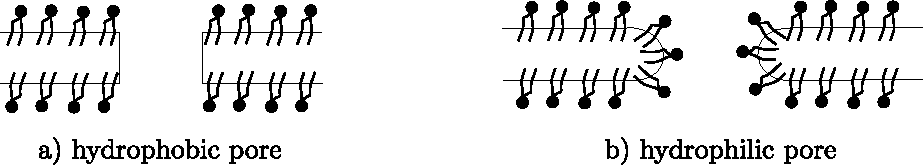
\includegraphics[scale=0.8]{pics/pores.pdf}
	\caption{Types of pores in lipid membrane}
	\label{fig:pores}
\end{figure}
%\begin{tikzpicture}
%\begin{axis}
%\addplot3[surf]
%table {data.dat};
%\end{axis}
%\end{tikzpicture}
The life time of the hydrophobic pores is in the order of the lipid fluctuations. Therefore, it is assumed that they are only intermediate stages in the formation of hydrophilic pores which are more stable and larger in size \citep{glaser1988reversible}. In this paper the intermediate stage of hydrophobic pores is neglected.

The mechanism of hydrophilic pores formation/annihilation is described by two competitive deriving force: the energy per length along the pore edges $\gamma$, we call it line tension, and the membrane tension or the energy per area of the membrane of a flat pore-free membrane $\sigma_0$ where it is simply called the surface tension. The energy of transient pore $\Delta W_{p}$ is usually given for a single pore with radius of $R$:
\begin{equation}
	\Delta W_{p}(R)=2\,\pi\,\gamma\,R-\sigma_0\,\pi\,R^2
\end{equation}
One can simply generalize this for pore region instead of one pore and rewrite the free energy equation in the form of two integrals. The first integral is the interracial contribution due to line tension $\gamma$ acting on the pore edges $\partial\Gamma$, and the second integral is the surface tension contribution to the porated area $\Gamma_p$ of the lipid membrane:
\begin{equation}
	\Delta W_{p} = \oint_{\partial\Gamma}\gamma\,ds - \int_{\Gamma_p}\sigma_0\,dA
	\label{eqn:transientmodel}
\end{equation}
%\begin{figure}[H]
%	\centering
%	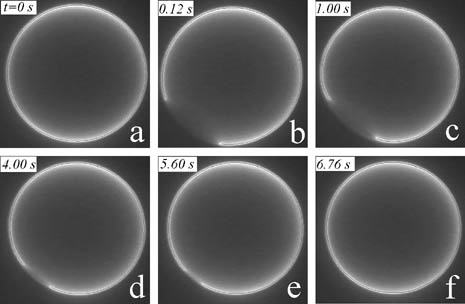
\includegraphics[scale=0.75]{pics/transient.jpg}
%	\label{fig:transient}
%	\caption{\footnotesize{Transient pore in a single vesicle}}
%\end{figure}
Surface tension $\sigma_0$ is responsible for appearance of transient pores in vesicles and lipid membranes. The surface tension for the membrane in relaxed state is very small. However, due to many reasons such as thermal fluctuations or increased hydrodynamic pressure inside the vesicle the membrane eventually becomes tense and pore formation occurs. After the pore formation and releasing the surface tension, pores will eventually reseal, the deriving force here is the line tension $\gamma$. In Figure \ref{fig:pore1} the opening and closing deriving forces are shown.


\subsection{Electroporation Model}
Many theories describing the electroporation process have surfaced in recent (and not so recent) years \citep{Weaver1996135,Zimmermann1974881,DeBruin19991213}. Electroporation is a dynamic phenomenon that depends on the local transmembrane voltage $U_{m}$ of the lipid part of the membrane. The induced voltage over the lipid membrane creates an extra surface tension $\sigma_{e}$ over the membrane in addition to the membrane tension $\sigma_0$ that already exists on the membrane. The overall surface tension then is $\sigma=\sigma_0+\sigma_e$ .
%There are two separate models to describe electroporation. The first model focuses in reproducing the temporal process of creation and evolution of pores, but the spatial distributions of the transmembrane voltage over the surface membrane, pore density, and other quantities are ignored. The second model solves the boundary value problem to calculate the spatial distribution of the transmembrane potential $U_m$. Models in this
%group compute the transmembrane potential assuming an intact membrane and use the magnitude of $U_m$ to assess the extend of electroporation.


\begin{figure}[H]
	\centering
	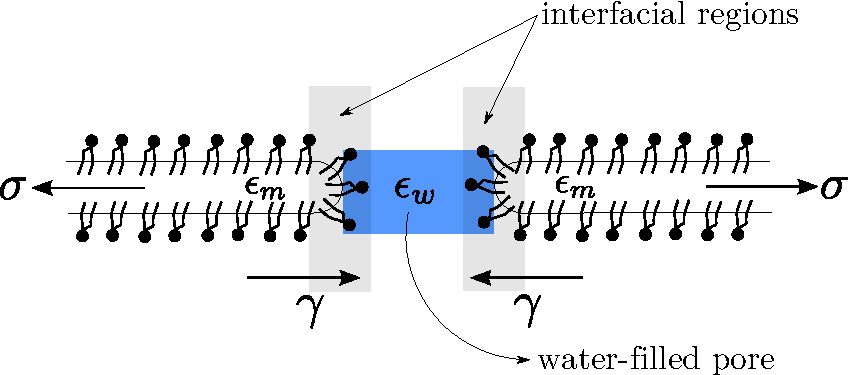
\includegraphics[scale=0.8]{pics/pore1_1.pdf}
	\caption{\footnotesize{Schematic of one water-filled pore in a lipid membrane}}
	\label{fig:pore1}
\end{figure}
Pore regions can be treated as having an energy associated with the change of its specific capacitance, $C_{LW}$, as lipid is replaced by water (a water-filled capacitor) shown in Figure (\ref{fig:pore1}). 
%It is been discussed that the voltage over a small pore is very close to the applied voltage $U_{p}\approx U=U_m$ due to the fact that the permittivity of pore is close to water (there is only \%10 difference) and the resistivity of a pore is large compared to spreading resistance \cite{Weaver1996135}. 
In the presence of a transmembrane electric field, the free energy of pore formation should be:
\begin{equation}
\Delta W_{p} = \oint_{\partial\Gamma}\gamma\,ds - \int_{\Gamma_p}\sigma_0\,dA-\int_{\Gamma_p}\sigma_e\,dA 
\label{eqn:poreenergy}
\end{equation}
The last term is an additional surface tension due to electric potential induced over the membrane surface. Electric surface tension defined as \cite{Weaver1996135}:
\begin{equation}
	\sigma_e=\frac{1}{2}\,C_{LW}\,\bar{U}_{m}^{2}
	\label{eqn:elecsurface}
\end{equation}
 Here $\bar{U}_{m}$ is the spatially averaged transmembrane voltage, 
%\begin{equation}
%\bar{U}=\frac{U_m\,A_m+U_p\,A_p}{A_m+A_p}\approx U_m\frac{A_m}{A}
%\end{equation}
%where the membrane voltage $U_m$ is the voltage across lipids and $U_p\approx0$ is the voltage across conductive pores. The area consists of lipid molecules is $A_m$ and the area filled with pores is $A_p$ where the total area of the lipid membrane is $A=A_m+A_p$. 
\begin{figure}[H]
	\centering
	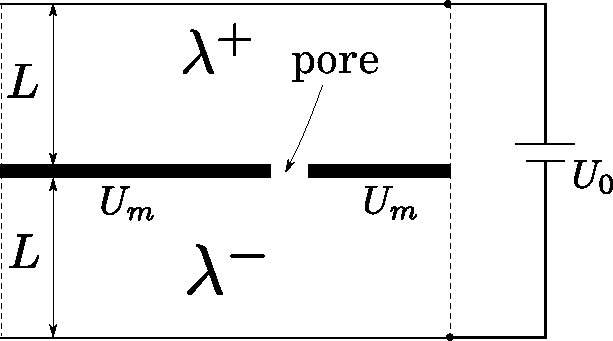
\includegraphics[scale=0.75]{pics/model0.pdf}
	\caption{A lipid membrane placed in a uniform electric field.}
\end{figure}
The membrane voltage $U_m$ can be obtained from solving electric field equation of the system:
\begin{equation}
	\nabla^{2}\Phi^{\pm}=0
\end{equation}
where $\mathbf{E}^{\pm}=-\nabla\Phi^{\pm}$ is the electric field. At the electrodes, the potential satisfies the boundary conditions $\Phi(x,y,\pm L,t)=\mp U_0/2$, conservation of normal currents requires
\begin{equation}
	C_m\,\frac{d\bar{U}_m}{dt}+G_m\bar{U}_{m} +I_{p}=\lambda^{\pm}\mathbf{n}\cdot\mathbf{E}^{\pm}
\end{equation}
where $U_m(t)=\Phi^{+}(x,y,0,t)-\Phi^{-}(x,y,0,t)$ is the membrane voltage and $\mathbf{n}$ is the unit normal vector. $G_m$ is the conductance of the lipid membrane and $I_p$ is the current density of pore regions:
\begin{equation}
I_p=\frac{\bar{U}_m}{R_{p}}
\label{Um}
\end{equation}
where $R_p=h/\lambda A_p$ is the pore resistance with $A_p$ being the area of the pore region and $\lambda$ is the conductivity of the solution filling the pore and $h$ is the thickness of the membrane.

At $t=0$, when the field is applied, the potential is assumed to be continuous, $\bar{U}_m(t=0)=0$. These system of equation can be solved numerically.
%\begin{equation}
%	U_m = U_0\,\left(1-\exp({-t/\tau_m}) \right)
%\end{equation}
%the time scale $\tau_m$ is defined as follow:
%\begin{equation}
%	\tau_m=C_m\,L\,\frac{(\lambda^{-} + \lambda^{+})}{(\lambda^{+}\,\lambda^{-})}
%\end{equation}
where $\lambda^{\pm}$ is the interior and exterior electrolyte (i.e. water) conductivity. This solution is the result of solving the electric field system of equation and the leaky dielectric assumption applied on the lipid membrane. Details are given in Appendix A.

The change of the pore's specific capacitance as water displaces lipid to form a pore is simply 
\begin{equation}
C_{LW}=\left(\frac{\epsilon_w}{\epsilon_m}-1\right)\,C_m
\end{equation}
Here $\epsilon_w=K_w\,\epsilon_0$ is the permittivity of water and $\epsilon_m=K_m\,\epsilon_0$ is the permittivity of lipid membrane, and $C_m$ is the constant capacitance per area of a pore free membrane, i.e $C_m=\epsilon_m/h$ where $h$ is the thickness of the membrane. Typically $K_w=80$ and $K_m=2$, so when the potential $\bar{U}$ increases $\Delta W$ decreases which means pore nucleation is more desirable.

%-------------------------------------------------%
\section{Diffuse Interface Model}
%-------------------------------------------------%
We are adopting the first order phase transition model. This model implies that broken membrane states (pore phase) have lower free energy than intact membrane states (lipid phase). This concept first introduced on the study of stability of soap films \cite{deryagin1962theory, derjaguin1981theory}. This approach assumes at the presence of electric field the membrane breakdown occurs because it is energetically more desirable i.e. transitioning to more stable phase.
%\subsection{Sharp Interface Model}
%Here we start with the free energy functional of an open lipid membrane with free exposed edges: \cite{PhysRevE.68.061915, PhysRevE.66.021607}
%\begin{equation}
%E = \int_{\Gamma}\frac{1}{2}\,\kappa\,\left(H-C_{0}\right)^{2}+\int_{\Gamma}\bar{\kappa}\,K+\int_{\Gamma}\sigma+\oint_{\partial\Gamma}\gamma
%\label{eqn:func1}
%\end{equation}
%where $H$ is the mean curvature, $C_0$ is called the spontaneous curvature, $\kappa$ is the bending rigidity, $\bar{\kappa}$ is the Gaussian bending rigidity, $\sigma$ is the surface tension and $\gamma$ is the line tension.
\begin{figure}[H]
	\centering
	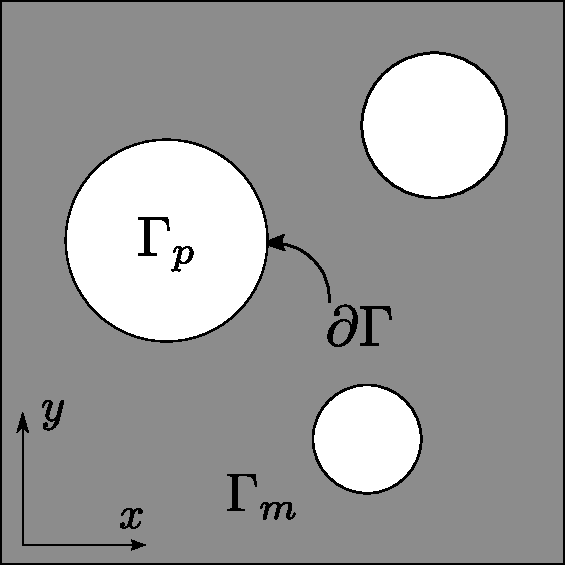
\includegraphics[scale=0.5]{pics/model1_2.pdf}
	\caption{\footnotesize{Schematic of the whole domain $\Gamma = \Gamma_m \cup \partial\Gamma \cup \Gamma_p$. $\Gamma_m$ indicates lipid membrane phase, $\Gamma_p$ is the pore phase, and $\partial\Gamma$ is the interface }}
	\label{fig:model1}
\end{figure}
%The first two integrals accounts for the curvature energy of the lipid membrane. The third integral accounts for the surface energy and the last one accounts for line energy due to exposed edges of the open lipid membrane. The shape equation then derived by taking the first variational derivative of Equation (\ref{eqn:func1}) \cite{PhysRevE.68.061915},
%\begin{equation}
%\delta\,F=-2\,\sigma\,H+\kappa\,\left(2\,H+C_{0}\right)\,\left(2\,h^{2}-C_{0}\,H-2\,K\right)+\kappa\,%\nabla_{\Gamma}^{2}\left(2\,H\right)=0
%\label{eqn:derv2}
%\end{equation}
%and on the boundaries ($\partial\Gamma$):
%\begin{equation}
%\bar{\kappa}\left(2\,H+C_{0}\right)+\bar{\kappa}\,k_{n}=0,
%\label{eqn:edgebc1}
%\end{equation}
%\begin{equation}
%-\kappa\,\mathbf{e_{2}}\cdot\nabla\left(2\,H\right) + \gamma\,k_{n}+\bar{\kappa}\,\frac{d\tau_{g}}{dS}=0,
%\label{eqn:edgebc2}
%\end{equation}
%\begin{equation}
%\frac{\kappa}{2}\,\left(2\,H+C_{0}\right)^{2}+\bar{\kappa}\,K+\sigma+\gamma\,k_{g}=0,
%\label{eqn:edgebc3}
%\end{equation}
%where $k_{n}$, $k_{g}$ and $\tau_{g}$ are the normal curvature, geodesic curvature and torsion curvature, respectively. In the case of a flat lipid membrane such as the one shown in Figure (\ref{fig:model1}) the curvature components in $z$ direction are all zero. The normal curvature $k_n$ over the boundaries of $\partial\Gamma$ and the mean curvature $H$ and also Gaussian curvature $K$ over $\Gamma$ vanish. Also the torsion curvature $\tau$ for planar surface vanishes too where the total curvature $k=\sqrt{k_n^2+k_g^2}$ is non-zero. The equations will decrease to:
%\begin{equation}
%\sigma+\gamma\,k_{g}=0
%\end{equation}
%The hydrodynamic effects over the lipid membrane sheet is neglected here. %\cite{:/content/aip/journal/pof2/23/4/10.1063/1.3567276} investigated the instability of lipid membrane in their one-dimensional model and the role of electrohydrodynamic that modulates the lipid density and shape fluctuations were taken into account.
%Here the main assumption is that the flat lipid bilayer sheet remains flat and all the time. The role of spontaneous curvature $C_0$ that determines the shape of lipid membrane is neglected.
%The energy of the pore is then defined as:
%\begin{equation}
%	\Delta W_p = \oint_{\partial\Omega}\gamma\,ds-\int_{\Omega^{p}}\sigma_{total}\,dA
%	\label{eqn:energyofpore2}
%\end{equation}
%where $\sigma_{total}=\sigma+$
The phase-field function $\phi$ is defined for two states $\phi=1$ for lipid membrane (grey regions in Figure \ref{fig:model1}) and $\phi=0$ for pores (voids in Figure \ref{fig:model1}), and the phase interfaces are replaced by thin layer across which $\phi$ changes its value between $0$ to $1$. The line tension energy in Equation \ref{eqn:poreenergy} can be replaced with Ginzburg-Landau energy form \cite{elliott2010surface,du2011phase}. Therefore,
\begin{equation}
	\Delta W_p\left[\phi\right]=\int_{\Gamma}\bar{\gamma}\,\left(\frac{\varepsilon}{2}|\nabla\phi|^{2}+\frac{1}{\varepsilon}\,g\left(\phi\right) \right)-\int_{\Gamma}\sigma\left(1-H(\phi)\right)c_0
	\label{eqn:func2}
\end{equation}
where $g(\phi)=\frac{1}{4}\phi^2(1-\phi)^2$ is a double-well potential function and $\varepsilon$ a small length scale. The coefficient $\bar{\gamma}$ is related to the line tension coefficient $\gamma$ by
\begin{equation}
	\bar{\gamma}=\frac{3}{4}\,\gamma
	\label{eqn:tensioncoeff}
\end{equation}
The function $H(\phi)$ is the Heaviside or the step function. The smooth Heaviside function $H(\phi)\approx\frac{1}{2}+\frac{1}{2}\,\tanh\left(k\,(\phi-\frac{1}{2})\right)$ were chosen in order to utilize the better separation behaviour of two phases where larger $k$ corresponds to a sharper transition at $\phi=1/2$. The coefficient $c_0$ is the area correction coefficient in order to keep the area constant
\begin{equation}
	c_0=\frac{\int_\Gamma(1-\phi)}{\int_{\Gamma}\left(1-H(\phi)\right)}
\end{equation}
The Allen-Cahn type dynamic formulation can be obtained from the energy functional in Equation \ref{eqn:func2}:
\begin{align}
		\frac{\partial\phi}{\partial t}&=-M\,\frac{\delta\Delta W_p}{\delta\phi}+\eta(\mathbf{x},t) \nonumber \\
		&=-M\left(-\bar{\gamma}\,\varepsilon\,\nabla^2\phi+\frac{\bar{\gamma}}{\varepsilon}\,g'(\phi)  + \sigma\,\delta(\phi)\,c_0\right)+\eta(\mathbf{x},t)
		\label{pf}
\end{align}
where $g'(\phi)=\frac{1}{2}\left(\phi-3\phi^2+2\phi^3\right)$ and also the Dirac's delta function $\delta(\phi)=dH(\phi)/d\phi$ is the derivative of Heaviside function. $M$ is related to the time scale for atomic rearrangement from the disordered phase to ordered one called the mobility coefficient where can be related to the diffusion coefficient $D$ and temperature $T$ by the Einstein relation $D=M\,k_B T$, and the coefficient $k_B=\unit[4.11\times10^{-12}]{J}$ is called is the Boltzman's constant, and $\eta(\mathbf{x},t)$ is the stochastic noise due to thermal fluctiuations and satisfies the relation:
\begin{equation}
\langle\eta(\mathbf{x},t)\ \eta(\mathbf{\bar{x}},\bar{t})\rangle=2M\,k_B T\,\delta(\mathbf{x}-\mathbf{\bar{x}})\,\delta(t-\bar{t})
\end{equation}
\section{Numerical Method}
We introduce the following non-dimensional variables:
\begin{equation*}
\mathbf{x}'=\frac{\mathbf{x}}{l}, \quad t'=\frac{t}{\tau}
\end{equation*}
where $l$ is a characteristic length of the membrane and $\tau=l^2/D$ is the characteristic time associated with diffusion of the lipid molecules. Where $D$ is the diffusion coefficient of lipid membrane and $D=M\,k_B T$. Also the dimensionless surface and line tension can be acquired:
\begin{equation*}
\gamma'=\frac{\gamma\,l}{k_B T}, \quad \sigma'=\frac{\sigma\,l^2}{k_B T}
\end{equation*}
 The non-dimensionalized and discretized form of Equation \ref{pf} is going to be:
\begin{equation}
	\frac{\phi^{n+1}_{i,\ j}-\phi^{n}_{i,\ j}}{\Delta{t'}}={\gamma'}\,{\varepsilon'}\bar{\nabla}^2\phi^{n}_{i,\ j}-\frac{{\gamma}'}{\varepsilon'}
\,g'(\phi^{n}_{i,\ j})-{\sigma}'\,\delta(\phi^{n}_{i,\ j})\,c_0+{\eta}'(\mathbf{{x'}},{t'})
\end{equation}
The form of discrete Laplacian operator $\bar{\nabla}^2$ is used where it introduced first by Oono and Puri:
\begin{equation}
\begin{split}
\bar{\nabla}^2{\phi^{n}_{i,\ j}}=\frac{\phi_{i+1,\ j}+\phi_{i-1,\ j}+\phi_{i,\ j+1}+\phi_{i,\ j-1}}{2\,{\Delta x'}^{2}}\\
+\frac{\phi_{i+1,\ j+1}+\phi_{i-1,\ j+1}+\phi_{i+1,\ j-1}+\phi_{i-1,\ j-1}}{4\,{\Delta x'}^{2}}\\
-\frac{3\,\phi_{i,\ j}}{{\Delta x'}^2}
\end{split}
\end{equation}
Take the lipid molecules the line tension $\gamma$ is reported to be between $\unit[10]{pN}$ to $\unit[30]{pN}$. We choose the characteristic length $l$ to be $k_B T/\gamma$. This gives 
\newpage
\appendix
\section{Solution to Electric Field}

\newpage
\bibliographystyle{plain}
\bibliography{ref}



\end{document}